\documentclass[10pt,twocolumn,letterpaper]{article}

\usepackage{cvpr}
\usepackage{times}
\usepackage{epsfig}
\usepackage{graphicx}
\usepackage{amsmath}
\usepackage{amssymb}

% Include other packages here, before hyperref.

% If you comment hyperref and then uncomment it, you should delete
% egpaper.aux before re-running latex.  (Or just hit 'q' on the first latex
% run, let it finish, and you should be clear).
\usepackage[breaklinks=true,bookmarks=false]{hyperref}

\cvprfinalcopy % *** Uncomment this line for the final submission

\def\cvprPaperID{****} % *** Enter the CVPR Paper ID here
\def\httilde{\mbox{\tt\raisebox{-.5ex}{\symbol{126}}}}

% Pages are numbered in submission mode, and unnumbered in camera-ready
%\ifcvprfinal\pagestyle{empty}\fi
\setcounter{page}{1}
\begin{document}

%%%%%%%%% TITLE
\title{Explainable Recommendation System Overview}

\author{Zihao Li\\
University of Chinese Academy of Sciences\\
Technology and Engineering Center for Space Utilization, Chinese Academy of Sciences\\ 
{\tt\small lizihao182@mails.ucas.ac.cn}
% For a paper whose authors are all at the same institution,
% omit the following lines up until the closing ``}''.
% Additional authors and addresses can be added with ``\and'',
% just like the second author.
% To save space, use either the email address or home page, not both
}

\maketitle
%\thispagestyle{empty}

%%%%%%%%% ABSTRACT
\begin{abstract}
   With e-commerce developed prosperity, the recommendation system is used wildly in our daily life. At the meantime, the explainable recommendation system has been attending vitally by researchers. In this paper, we emphasize the significances and necessities of explainable recommendation. After that, we review the latest related works before the year 2019. Furthermore, we illuminate the two main methods: matrix factorization based and neural network based, and then introducing some common models respectively, such as knowledge-based, association-based, topic-based, etc. In addition, we compare the key ideas of these two mainstream models and analysis the major research direction of explainable recommendation system nowadays. Finally, we point out how to combine with the large external auxiliary information and prior knowledge effectively and how to design a more elaborative model faced with differenet scenarios will be the hot topic for explainable recommendation system.
\end{abstract}

%%%%%%%%% BODY TEXT
\section{Introduction}
Based on internet technology developed rapidly, e-commerce has already penetrated in this modern society. Amazon, Yelp, IMDB, Youtube, such as these products or services facilitate and enrich our daily life extremely. Simultaneously, these tools collective our data and information moment by moment. Standing on the merchants' sides, how to utilize the accumulation user's demographic information and behavior data, like text reviews, geographic information, social information, items attributes as well, to increase the click-through rate (CTR) of applications and user engagement to increase their profits, which will be an essential problem. As for users, how can we find the products that meet our requirements quickly and precisely? It is also an enormous challenge. Therefore, the propose of the recommendation system is to extract the user's points of interest (POI) or substantial POI and aiming at the different interests to help the user find the better items form the magnanimous data and realize the individual recommendation. Besides, another objective of the recommendation system is to release or solve the problem of information overload in the present time of information explosion. Very recently, the researchers pay more and more attention to the explainable recommendation system, that is to say, not only should we focus on the accuracy and recall of recommendation lists, but we also should shed light on the users purchase or click behavior, explore and provide the reason of recommendation results. In this way, it can help the engineer to improve the system and provide a better service. In this work, we will illuminate some different types of explainable recommendation system and summarize the common framework of future research.

%-------------------------------------------------------------------------
\subsection{Explainable Recommendation System}
Explainable recommendation system applied various kind of scenarios, for instance, e-commerce, social communication, information retrieval, multimedia recommendations as well as some exclusive areas. E-commerce product recommendation is a typical scenario of explainable recommendation, like Amazon e-commerce, Tmall e-commerce, JD e-commerce as well. Besides, the meal ordering platform, hotel and restaurant websites and commercial advertisement also need an explainable recommendation. The explainable recommendation can help to improve transparency, trustworthiness, and persuasiveness and making the process of decision faster and easier. Social recommendation, such as friend recommendation, blogs, news, music, books recommendation will also refer to social information. Based on this assumption that our friends may have a similar POI of me, explainability of the social recommendation system is critically important to increase the persuasion of recommendation lists. Thus we can leverage Twitter, Facebook and Weibo data to provide the recommendation. Multimedia recommendation mainly refers to video recommendation like YouTube, MovieLens. Above all, if we face the retrieve task and at the same time there exists information overload problem, we can consider using the recommendation system.

Classical recommendation models, like user-based or item-based Collaborative filtering (CF) (J. Herlocker et al. 2000): matrix factorization, neural networks: Restricted Boltzmann Machine (RBM) (Abdollahi B et al. 2016), probability graphic model: Latent Dirichlet Allocation (LDA) (Blei D M et al. 2003), Probabilistic latent semantic analysis (pLSA) topic models (Eisenstein J et al. 2010, Hong L et al. 2012, Sizov S. 2010, Yuan Q et al. 2013), aforementioned methods project the users and items intuitive features or attributes into a high-dimensional internal and invisible representation, such an embedding process makes the models be complex black-boxes, and hard to explain. The explainable recommendation system tempts to clarify why they provide the recommendation to users, in addition, the explainable recommendation aims to construct an interpretable model to work and think like a human way. The most of explainable recommendation systems are called post-hoc models, in the next section, we will give a big picture of two categories for the explainable recommendation methods: MF-based and NN-based, which will help readers get a clearly and exactly understanding of this problem.

\subsection{Traditional Method}
{\bf Matrix Factorization.} Generally speaking the basic idea of matrix Factorization or latent factor models, neighborhood-based models are collaborative filtering. This means the similar people are likely to similar items, or similar items may have a good chance to be interested in different users. Therefore, we can select $N$ nearest (most similar) neighbors of items and users by the users' historical behaviors data and recommend. For example, if user A like item a, and user B is similar to user A, then user B is more likely to like item a, $<$ A like a, A similar B $\to$ B like a $>$, and if user A like item a, item a is similar to item b, then user A is possible like item b, $<$ A like a, a similar b $\to$ A like b $>$. Above-mentioned methods are user-based and item-based CF. Relying on this clearly motivation, we can design the user-item matrix by the historical behaviors data, however this matrix will be huge and sparse definitely, thus matrix factorization can be used to construct two small and dense matrixes which represent the users' latent representation and items' latent representation respectively to fit or modification the raw matrix. The model shown in {\bf Figure 1}, applying the MF, we can find the top items of user interest and recommend. Suppose the score of user $u$ to the item $i$ is $r_{ui}$, and the predicted score by MF is $\hat{r}_{ui}$, then we have this objection function:

\noindent
\begin{equation*}
	\begin{split}
	L=&\sum_{(u,i)\in K}(r_{ui}-\hat{r}_{ui})^2=\sum_{(u,i)\in K}(r_{ui}-\sum_{k=1}^{K}p_{u,k}q_{i,k})^2\\
	&+\lambda (||p_u||^2+||q_i||^2)
	\end{split}\tag{1}
\end{equation*}
where $p_{u,k}$ and $q_{i,k}$ are the user and item latent representation, $\lambda (||p_u||^2+||q_i||^2)$ is the regularizer to prevent overfitting. To changing the regularizer or merge more auxiliary information or consider the pairwise representation, we will extend a series of models, such as BPR (Rendle, 2009), NMF (Zhang, 2006), SVD++ (Koren, 2008), etc. 
\begin{figure}
	\begin{center}
		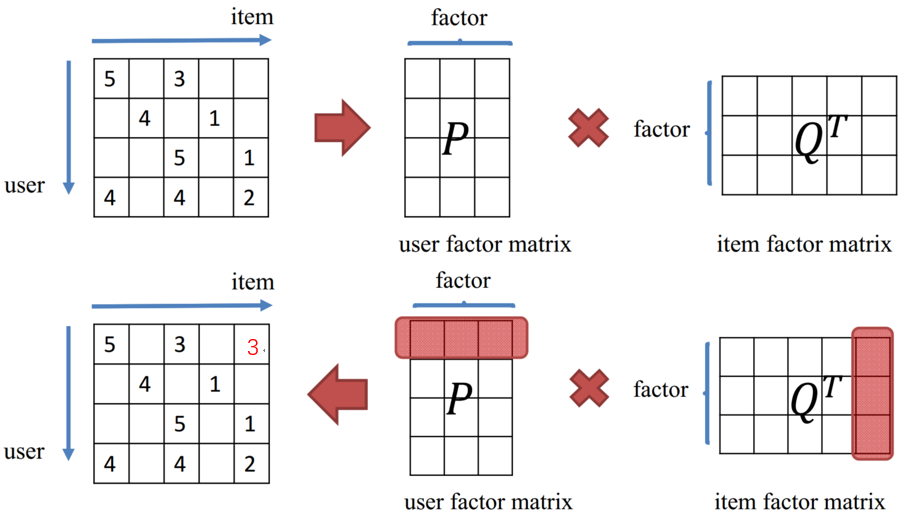
\includegraphics[width=0.8\linewidth]{mf.png}
	\end{center}
	\caption{The user-item matrix can be factorized as two small matrix: user factor matrix $P$ and item factor matrix $Q^T$, thus based on the matrix multiplication, we can complement the raw matrix and recommend.}
	\label{fig:long}
	\label{fig:onecol}
\end{figure}

{\bf Latent factor model.} Latent factor model (LFM) can be understood as probabilistic matrix factorization or probability graphical model, which is the original method from the topic model in text mining regions, like LSI, pLSA, and LDA. Since Netflix Prize competition organized, the LFM gradually becomes a popular algorithm and now it is a major model in recommendation system. The probabilistic graphics model assume the user's interests or item attributes obey a certain of probability distribution such as Gaussian distribution, and the distribution can be observed by the review texts and other factors. These explicit factors probability is easy to be counted, while the latent factors are often coupled together, so we usually calculate the maximum likelihood through the EM algorithm, MCMC (Markov Chain Monte Carlo), or leverage gradient descent methods directly. {\bf Figure 2} shows the graphical model for constrained PMF (Ruslan et al, 2007). The $R_{ij}$ represents the preference of user $i$ to item $j$, $U_i, V_j$ represent the latent factor of users and items, and both of them obey the Gaussian distribution, $I_i$ is an indicator function, if $R_{ij}$ exists it will be 1, otherwise it's 0. $Y$ is the original unrevised $U$ and $W$ latent similarity constraint matrix, the values reflect the item's influence to the user, which is also Gaussian distribution. According to this framework, We can introduce more latent factors, like item attributes, sentiment information, and geographic information, to complete the graphics model and improve the results of the recommendation.
\begin{figure}
	\begin{center}
		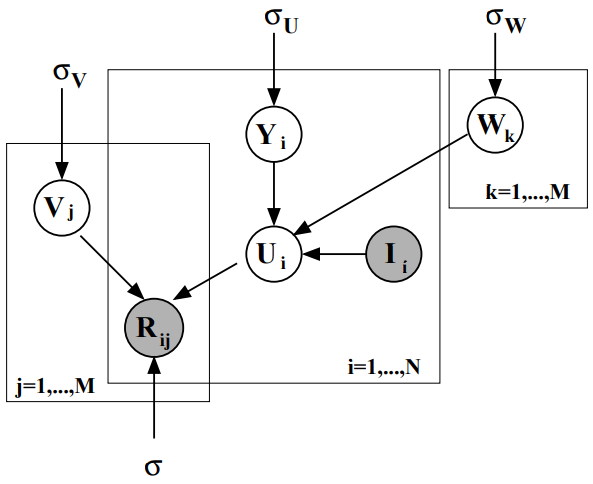
\includegraphics[width=0.8\linewidth]{gm.png}
	\end{center}
	\caption{The panel shows the graphical model for constrained PMF. The user's preference for items $R_{ij}$ is determined by the factorized vectorized vectors of users and items which are in line with the Gaussian distributions.}
	\label{fig:long}
	\label{fig:onecol}
\end{figure}

{\bf RBM.} RBM (Restricted Boltzmann machine) can be recognized as a classical shallow neural network or an encoder-decoder machine, which transform the recommendation problem into a prediction problem, or a regression problem (Ruslan et al, 2007). The inputs of the model are the feature embedding of items and users the output is the prediction scores for different users about different items. As for the features selection and model's design, there are a great number of works, like Wide $\&$ Deep network (Cheng et al, 2016). 

{\bf Others.} There are many other recommendation methods. Correlation-based, distance based. This kind of methods calculates the similarity of the items among different attributes through Cosine, Pearson correlation, OLS coefficient, Euclidean distance, Minkowski distance, etc. As above the item-based CF and correlation-based methods, both of them realize the recommendation by the similarity of different items, however they have a clear distinction, CF-based model is more based on the user's behavior data and does not care about the items intrinsic properties, while the correlation-based model focuses on the attributes of items. Graph-based models consider the user-items relation as a bipartite graph then through the nodes or edges weights and links to recommend, consequently the graph model: Shortes Path, Random Walk, Item Rank can be leverage in recommendation problem. Cluster-based, "Birds of a feather flock together", intuitively we can recommend the same items to the cluster users, meanwhile method for grouping similar items in high dimensional spaces, thus we can combine the cluster method with hashing, like LSH (Locality Sensitive Hashing) for clustering (Nima et al, 2013). In fact, the CF also can be regarded as a clustering method and LDA is also a clustering algorithm in nature.

The classical methods have been proved the great power in the recommendation system, especially for the matrix fraction and RBM models which were the best solutions in Netflix Prize competition. Nevertheless, the traditional methods can not give a convictive explanation to the recommendation, which is disadvantageous to the development of the recommendation system. A transparent and explainable recommendation is the main direction of current research.

\section{Related Work}
Study shows that the explainable recommendation system can increase the acceptance of proposed products, convincing the users to purchase the recommended items, expediting the process of making decisions, and even enhance the trust to the system as a whole (Herlocker et al, 2000). In this section, we will give a brief introduction to the latest works of explainable recommendation system from different classification.

\subsection{Neural Network}
Neural networks consider the recommendation as a prediction task, the pipeline is that embedding the user's and item's features or attributes, then feeding to the neural network and obtaining the scores of candidate sets. About the features selection, there have a lot of works, for instance, decision tree based, wide and deep networks. As for neural networks structures, we can integrate the attention mechanism, memory networks, reinforcement learning, etc. Besides, we can also incorporate external information, such as knowledge-based, user's and item's review, social network, sentiments, contextual information, regions to enhance the explanation of the recommendation system. 

{\bf Tree-enhanced Embedding Model.} Collaborative filtering leverages the users and items feature to building a personalized recommendation system, however, these features are high-dimension and invisible, thus it's unexplainable. On the other side, based on the divide-and-conquer strategy, the decision tree has a definite and visible decision-making or feature selection process ({\bf Figure 3.}), therefore, we can leverage the selected features to training a network and realize the recommendation. According to this simple idea, Tree-enhanced Embedding Model (Wang et al, 2018) applied the GBDT (Gradient Boosting Decision Tree) as the precursor work of attributes selection, then feed the  user, item attributes embedding and user-item ids embedding into the attention network, and aimed at different user offer personalized recommendation ({\bf Figure 4.}), attributing to the decision tree, we can also provide a reasonable explanation for the recommendation results.
\begin{figure}
	\begin{center}
		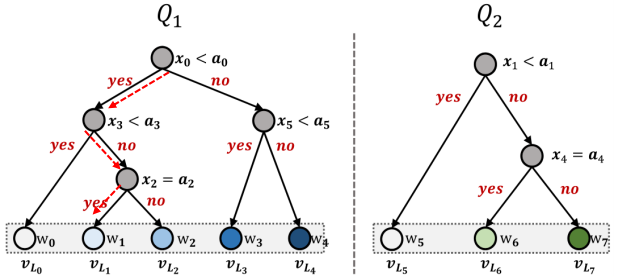
\includegraphics[width=0.8\linewidth]{TEM_1.png}
	\end{center}
	\caption{The process of feature selection in GBDT model.}
	\label{fig:long}
	\label{fig:onecol}
\end{figure}
\begin{figure}
	\begin{center}
		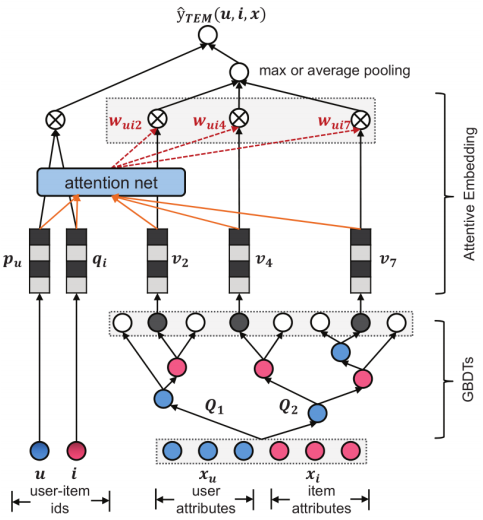
\includegraphics[width=0.8\linewidth]{TEM_2.png}
	\end{center}
	\caption{TEM framework. Leveraging the GBDT to select the item and user attributes then embedding, meanwhile, combining the user-item ids embedding feed into attention networks, this is because the different item will have the different attributes, and different uses will focus on different aspects and recommend.}
	\label{fig:long}
	\label{fig:onecol}
\end{figure}

{\bf RBM for CF.} The primitive RBM for recommendation system choose the item feature as input, and it leads to unexplainable. The CF can improve the explanation in some way, but the precision is lower than RBM. Consequently, how to combine the CF and RBM is a question. Behonoush (Behnoush et al, 2016) proposed taking the CF results as the input of RBM. Specifically, input the items' scores of user's neighbors determined by CF and the items' own scores to RBM to get recommendation scores, shows in {\bf Figure 5}.

\begin{figure}
	\begin{center}
		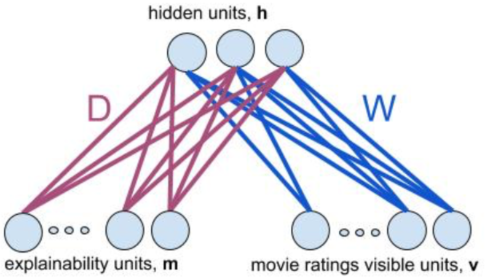
\includegraphics[width=0.8\linewidth]{RBM.png}
	\end{center}
	\caption{Conditional RBM for explainable. The explainability unit m means the user's neighbors score to this item, and the movie ratings visible unites is the inward scores.}
	\label{fig:long}
	\label{fig:onecol}
\end{figure}

{\bf Convolutional Sequence Embedding.} Typical sequence models such as RNN, LSTM, GRU will collect all the historical information to get the current output, however in recommendation task, not all the historical data are helpful to the decision right now. In addition, the purchase behavior doesn't have an obvious sequence features, maybe long before purchase behavior impacts the current behavior. Tang (Tang et al, 2018) proposed CNN to extract the items context connection and get the next recommendation lists.  Specifically, this paper combines user embedding, items embedding of horizon convolution filters and vertical convolution filters to get the prediction, Seen 
{\bf Figure 6}. To be attention, the author using horizontal convolutional and vertical convolutional layer to capture union-level patterns and point-level sequential patterns.  
\begin{figure*}
	\begin{center}
		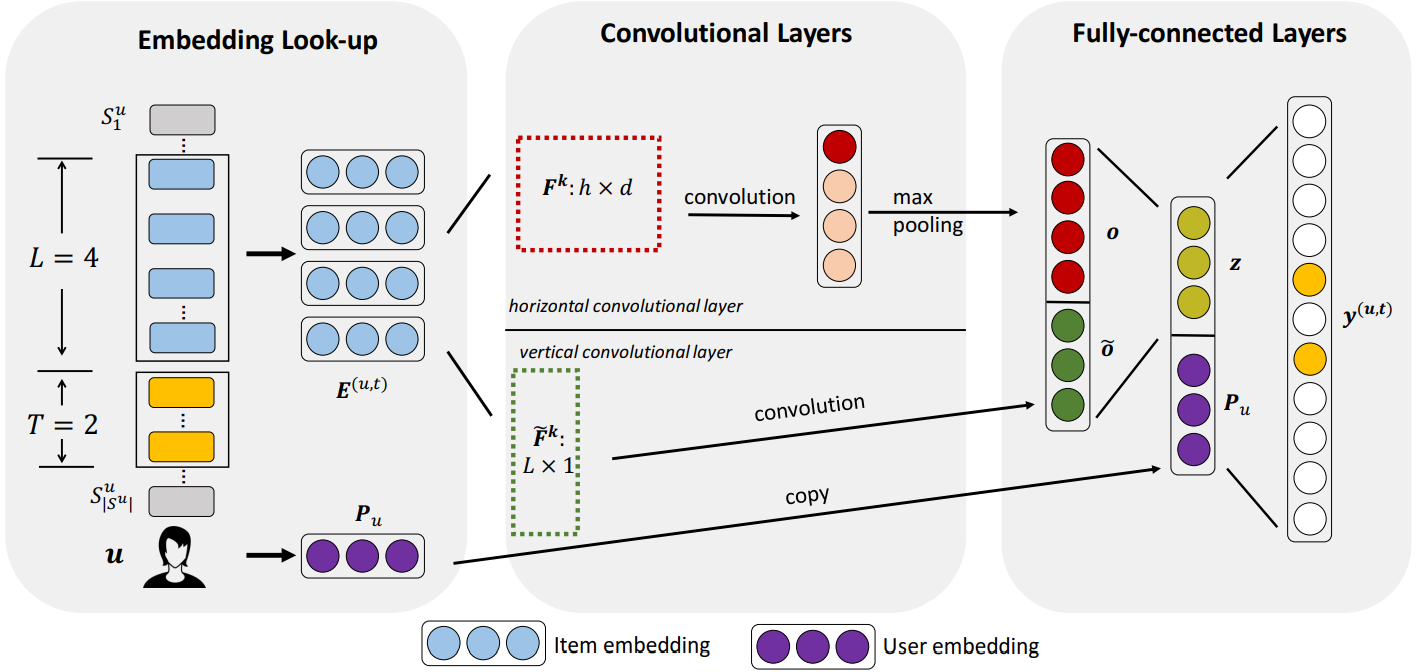
\includegraphics[width=.9\linewidth]{CNN.png}
	\end{center}
	\caption{The network architecture. The $S^u$ is the user sequence, we used previous 4 actions to predict the next 2 steps. $P_u$ is user embedding and $E^{(u,t)}$ is item embedding.}
	\label{fig:short}
\end{figure*}

{\bf Sequential Recommendation with User Memory Networks.} Different from the {\bf Convolutional Sequence Embedding}, this work considers the user action as a sequence model, but in order to select the history information better and avoid the latest action has a great impact, Chen (Chen et al, 2018) proposed the memory network on the basis of RNN. Memory network adopts the current item to decide what historical item information we should focus on (a routing mechanism), then combine the personal intrinsic embedding to conducting the prediction, and updating the memory matrix. In this paper, the author explores two memory network: item-based and feature-based, the item based model only embedded item, and update the memory by adding the current item embedding. While feature-based model attention to items' feature, embedding the item feature, and update the memory matrix drastically by the current item feature, Seen {\bf Figure 7}.  
\begin{figure*}
	\begin{center}
		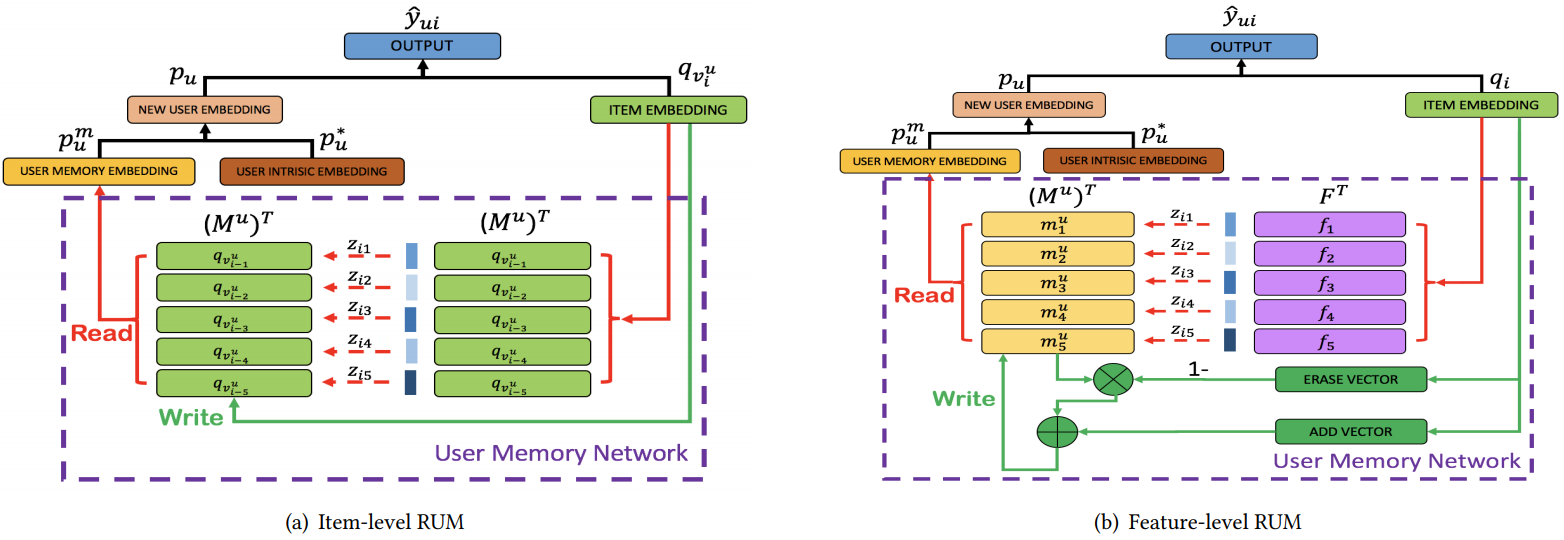
\includegraphics[width=.9\linewidth]{memory.png}
	\end{center}
	\caption{The user memory network and item memory network. $z_i$ is the memory weights or item embeddings.}
	\label{fig:short}
\end{figure*}

\subsection{Probability Graphic Model}
User's purchase decision influenced by a variety of factors this latent factors are coupled together, thus we can leverage the graphics model to mimic the user preference. By mining the latent factors inner relation and the causal relationship to predict, which makes the recommendation interpretable. 

{\bf Sentiment-Aspect-Region model.} Existing works do not consider the user item aspect incorporate, Zhao (Zhao et al, 2015) proposed SAR model to capture the user's POI from the three stands: sentiment-aspect-region at the same time, learning user preferences based on reviews, categories, and geolocations, building the graphics model to comment. {\bf Figure 8.} shows the graphics model, by the individual POI, category topical-region and individual user probability we can calculate the prediction score and recommend.   
\begin{figure}
	\begin{center}
		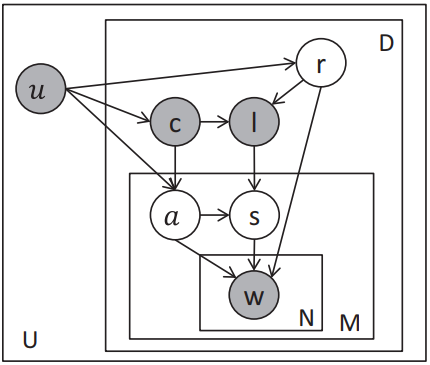
\includegraphics[width=0.8\linewidth]{SAR.png}
	\end{center}
	\caption{Sentiment-Aspect-Region Model. u, l, c, r, a, s, d, w, U, L, D, N, represent individual user, individual POI, category, topical-region, review, word, set of users, set of POIs, set of reviews, the number of sentences in a review and the number of words in a sentences. Their inner relation can be represented in this graphics mode.}
	\label{fig:long}
	\label{fig:onecol}
\end{figure}

{\bf Aspect-based Latent Factor Model.} In this work (Lin et al, 2016), the author fully extracts the reviews of the same items as well as users, leverage the latent factor vectors to solve the rating prediction, compare with the LFM, this model includes three latent factors. First one is a user-review matrix, where each element is word frequency in review texts of users, which exactly determine the category of items. The second one is an item-attribute matrix which includes item-property matrix and item-quality matrix. Item-property matrix reflects on the focus degree of the special aspects of products. Item-quality matrix shows the item quality by the counts of positive and negative words of reviews. In addition, combining the rating matrix to get rating prediction. From the {\bf Figure 9}, we can understand the relation of the latent factors in user content, item, and item quality matrix. The ALFM achieve the best accuracy in each category of Amazon dataset. Furthermore, it can also realize the "cold-start" problem effectively.
\begin{figure*}
	\begin{center}
		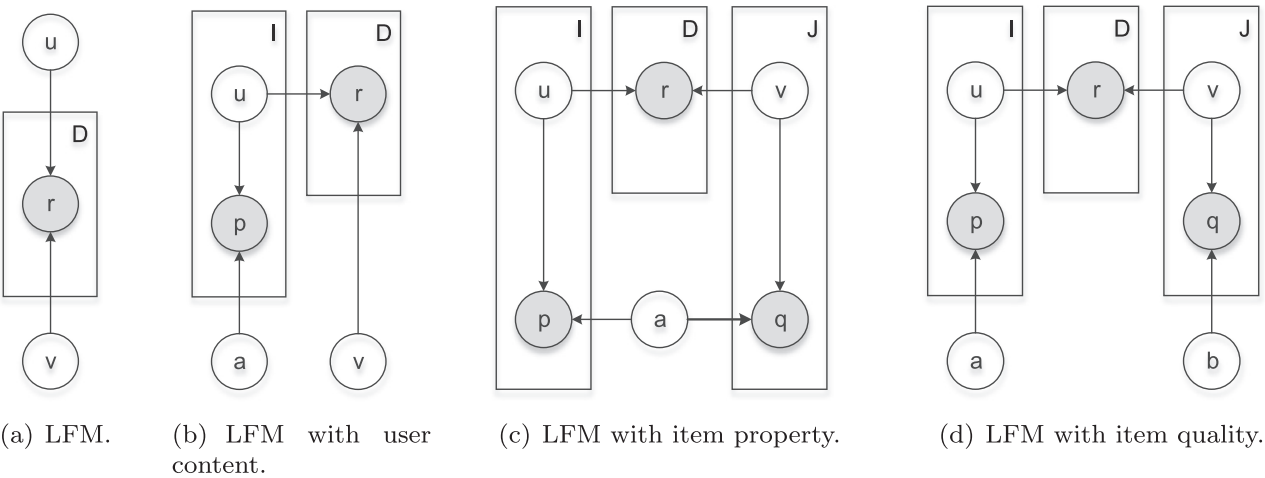
\includegraphics[width=.9\linewidth]{LFM.png}
	\end{center}
	\caption{LFM graphical model. r, u, v, p, a, q, b represent the rating, latent factor vector for user, latent factor vector for item, the feature of word in user's review, aspect distribution of word which represent semantic information learned from users’ review text, the feature of word in item's review, aspect distribution of word which represent semantic information learned from items’ review text. From the graphics model, we can obtain the connection between different factors.}
	\label{fig:short}
\end{figure*}

\subsection{Matrix Factorization}
Through factor a large space user-item score matrix as the product of two latent dense matrices, which represents the user and item representation respectively to comment. This is a common method, and we also can introduce the prior information to the project function as the bound terms to provide the explanation. This year many of works' inherit the idea, EFM (Zhang et al, 2014) is an excellent model in the early time. 

{\bf Overlapping Co-clustering Model.}There is no doubt that each item will have different aspect attributes and the user will not just care the single aspect of products ({\bf Figure 10}). But the traditional cluster allocates the item to a specific class, this approach is not appropriate clearly. Thus Reinhard (Reinhard et al, 2017) applied overlapping co-clustering to recommend, in this model the item can belong to various classes, which avoid the aforementioned defect. Specifically, we can appoint the number of classes at the time of parallel matrix factorization, thus the score of user-item pairwise can be calculated by the multi-MF. In addition, the author evidenced the algorithm has linear time complexity and can be applied to GPU easily.  
\begin{figure}
	\begin{center}
		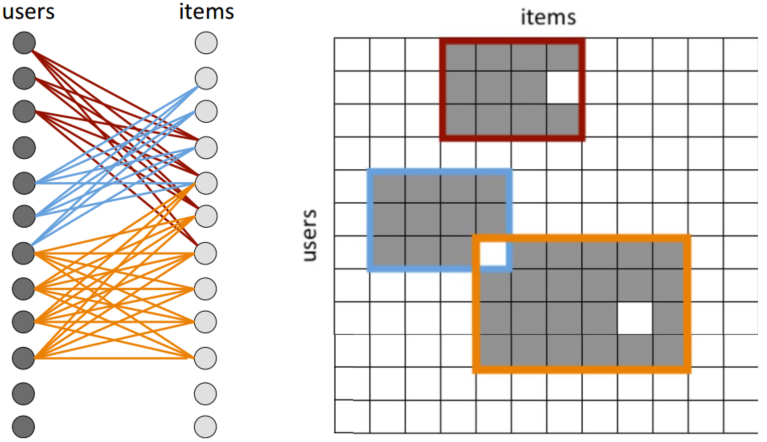
\includegraphics[width=0.8\linewidth]{co_cluster.png}
	\end{center}
	\caption{Example of overlapping user-item co-clusters, the white squares can belong to a different cluster, the blue and orange rectangular box.}
	\label{fig:long}
	\label{fig:onecol}
\end{figure}

{\bf AFM.} Even though different users give the same score of an item, they may have different reasons, that is to say, they may focus on different aspects of the item. Similarity, the different item may have the same scores, while the reasons are also various. Thus, Hou (Hou et al, 2019) proposed AMF (aspect matrix model) , consider the score prediction from the user and item aspects ({\bf Figure 11.}) And rely on matrix factorization get the user and item latent representations, then put them to the objection function as restrict condition. Furthermore, the author defines a SDA to evaluate the satisfaction degree of different items according to the different aspects. 

\begin{figure}
	\begin{center}
		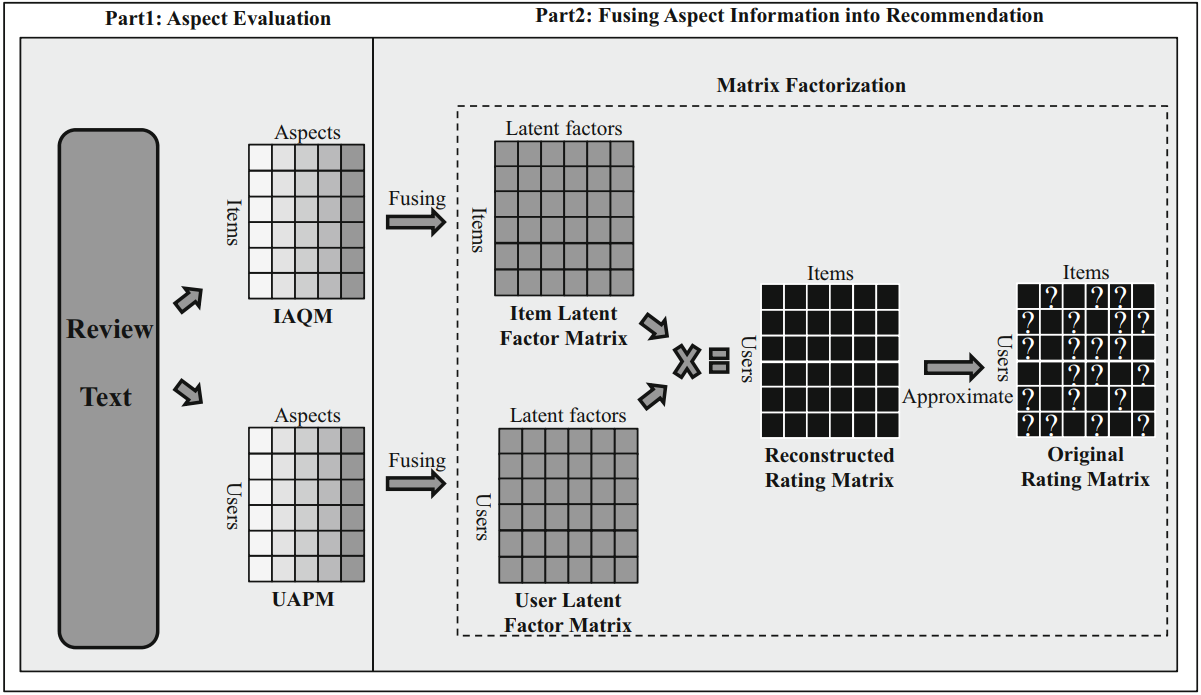
\includegraphics[width=0.8\linewidth]{EFM.png}
	\end{center}
	\caption{AMF, the review text can construct two matrices, IAQM and UAPM, which represent item latent factor matrix and user latent factor matrix respectively. After that, we can reconstruct the rating matrix and recommend.}
	\label{fig:long}
	\label{fig:onecol}
\end{figure}

{\bf Multi-Task Learning in Opinionated Text Data.} The user's preference for items, not only reflected by the score to the item, but the text review will also afford the concrete reason. Thus, based on text mining technology to extract the different aspects of items which the user focused ({\bf Figure 12}), and this method will have a good explanation for the recommendation. Therefore, we should model the refined aspect of items as well as the preference of items, Wang (Wang et al, 2018) develop multi-task learning via a joint tensor factorization to represent preference and opinion. Showing in {Figure 13}, a join tensor $\tilde{X}, Y^I, Y^U$ can be factorized to capture the user, item, feature and opinion latent representation.

\begin{figure}
	\begin{center}
		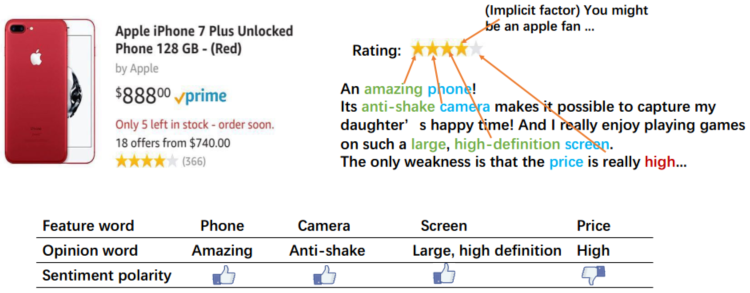
\includegraphics[width=0.8\linewidth]{multi_task_1.png}
	\end{center}
	\caption{Example of a star rating and a text review of a phone. Feature, opinion, preference is expressed clearly.}
	\label{fig:long}
	\label{fig:onecol}
\end{figure}

\begin{figure}
	\begin{center}
		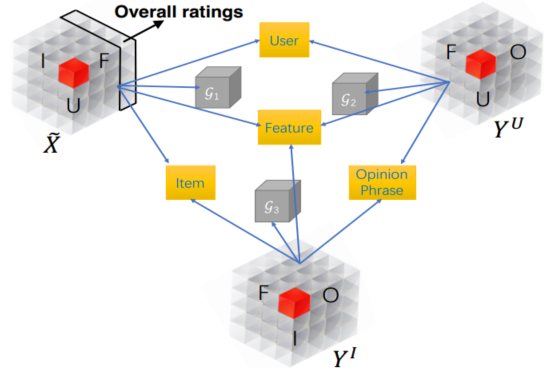
\includegraphics[width=0.8\linewidth]{multi_task_2.png}
	\end{center}
	\caption{Joint tensor decomposition scheme. I, F, U, O is an item, feature, user and opinion phrases latent factors.}
	\label{fig:long}
	\label{fig:onecol}
\end{figure}    

{\bf Post Hoc Interpretability of Latent Factor Models.} Through the nearest neighbor CF can recommend, nevertheless, this method ignores the items inner causal connection, while the association rules can promote the causal connection and realize the explanation recommendation. Thus we can consider these two models at the same time. Georgina (Georgina et al, 2018) according to the top N recommendation list provided by MF whilst leveraging the association rule to provide the interpretation ({\bf Figure 14}). This post-hoc approach contributes to the interpretability of recommendation. 
\begin{figure*}
	\begin{center}
		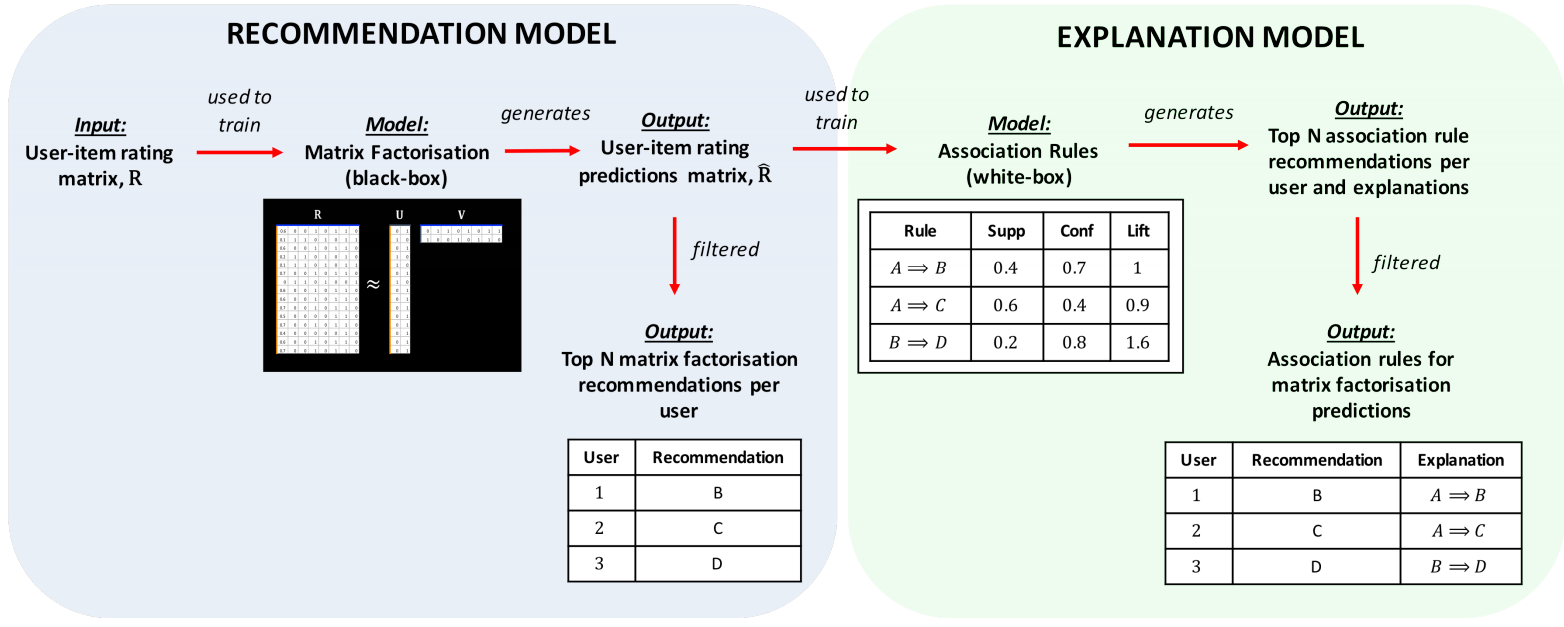
\includegraphics[width=.9\linewidth]{post_hog.png}
	\end{center}
	\caption{Schematic diagram of the proposed approach for generating an explanation model by training association rules on the output of a black-box matrix factorization recommendation model.}
	\label{fig:short}
\end{figure*}

{\bf Learning to Rank.} The common method use MSRE to evaluate the model, however in practice, we don't care the specific scores of recommendations, what we concern is the item rankings, showing in {\bf Figure 15}. Consequently, it's not suitable to apply RMSE to measure the models. Xu (Xu et al, 2016) promote relying on the user and item feature to learning a rank to improve the accuracy of the recommendation system. Generally, the model builds the preference pairs, transforming the absolute ranking to relative ranking to capture the order the rank of items.
\begin{figure}
	\begin{center}
		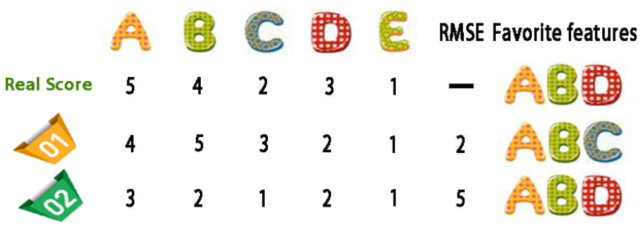
\includegraphics[width=0.8\linewidth]{learning_to_rank.png}
	\end{center}
	\caption{RMSE vs Ranking.}
	\label{fig:long}
	\label{fig:onecol}
\end{figure}

\subsection{Graphic Model}
Different from the probability graphic model, graphics model construct by the nodes and edges, the nodes are entities like users or items and edges represent the connection between adjacent nodes, for instance, social network, telecommunication network, knowledge graph which can be seen as a triple: head entity, tail entity, and relationship. We can depend on the neural network to learning the representation of entity and relation, such as TransE (Antoine et al, 2013), TransH (Wang et al, 2014), TransR (Lin et al, 2015). As for the recommendation system the item and user can be regarded as an entity, and the relation of attributes can establish the connection of different entities. Beyond that, we also can utilize the users' consuming behavior to establish the graph model.   

{\bf Entity-based Recommendations with Knowledge Graphs.} The items' attributes have the nature relation, based on knowledge graph and graph algorithm, we can map the items to the entity and find the relation by the attributes link, and recommending. For example user A like {\em The Razor's Edge}, the {\em The Razor's Edge} written by W. Somerset Maugham, and W. Somerset Maugham also wrote {\em The Moon and Sixpence}, thus we can recommend user A to {\em The Moon and Sixpence}. Directing by this idea Rose (Rose et al, 2017) introduce the knowledge graph to the recommendation task, and the recommendation list can be ensured by rules see {\bf Figure 16}.
\begin{figure}
	\begin{center}
		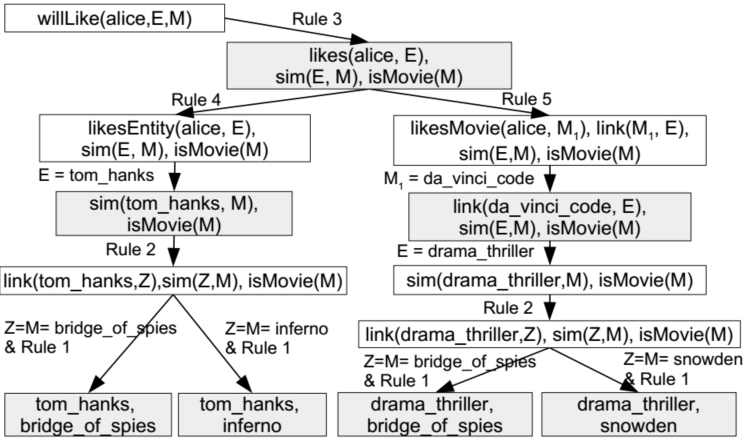
\includegraphics[width=0.8\linewidth]{KG.png}
	\end{center}
	\caption{Sample grounding for predicting likes.}
	\label{fig:long}
	\label{fig:onecol}
\end{figure}

{\bf A Social Explanation System.} Social data can be leveraged in the recommendation system. Lara (Lara et al, 2017) obtained three social factors: (1)Personality, that represents user predominant behavior according to her/his personality evaluation. (2) Tie strength that fits within a range of (0,1]. This value is automatically extracting features that act as predictors of tie strength in both users u’s and v’s Facebook profiles. (3) Satisfaction, that fits within a range of [0,1]. This value is computed by directly asking users their initial state and updated each time users report feedback through HappyMovie. Social information improves the preference for recommendation and makes it explainable.

{\bf TriRank.} Similar to knowledge, this leverage consider user, item and aspect to establish a tripartite graph, further He (He et al, 2015) decomposed the tripartite graph as two subnets, User-Item structure and  Item-Aspect structure, seen {\bf Figure 17}. Then according to smoothness implies local consistency (adjacent vertices have similar scores) and fitting encodes prior belief (the prediction shouldn't have a much deviation from the ground truth) to optimize the model. By considering the different aspects of items for each user, we can realize the explanation of recommendation and acquire the improve of accuracy.  
\begin{figure*}
	\begin{center}
		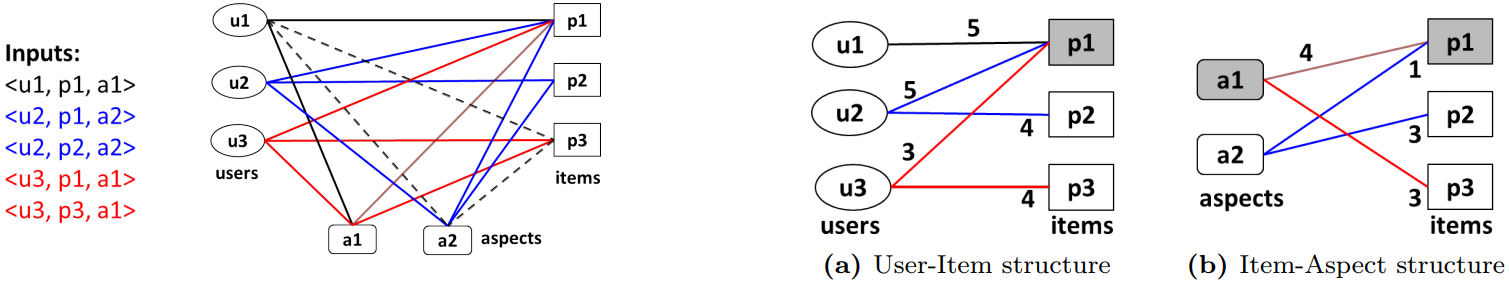
\includegraphics[width=0.9\linewidth]{TriRank.png}
	\end{center}
	\caption{Tripartite structure and decomposed graphs. u, a, p is user, item and aspect representation.}
	\label{fig:long}
	\label{fig:onecol}
\end{figure*}

\subsection{Explainable Recommendation Methods Summary}
From the {\bf table 1.}, we can clearly see that the primary methods of explainable recommendation are MF and NN, the principle data we utilize is user-review scores or rating and text reviews. Besides, we can also integrate the social information of users and knowledge graph of items.

\begin{table*}
\caption{A classification of above explainable recommendation models. About each method, we show two dimensions: the basic method and the auxiliary information.}
\begin{center}
\begin{tabular}{|c|c|c|} 
	\hline 
	Explainabel Recommendation System&Methodes&Auxialiary Information\\
	\hline  
	Wang et al, 2018&Neural Network&User and Item attributes\\
	\hline
	Behnoush et al, 2016&Neural Network&User-Item rating\\ 
	\hline
	Tang et al, 2018&Neural Network&User and Item record\\
	\hline
	Chen et al, 2018&Neural Network&User and Item review and record\\ 
	\hline
	Zhao et al, 2015&Probability Graphical Model&User and Item review\\
	\hline
	Lin et al, 2016&Probability Graphical Model&User and Item review\\
	\hline
	Reinhard et al, 2017&Matrix Factorization&User-Item purchase record\\
	\hline
	Hou et al, 2019&Matrix Factorization&User and Item review\\ 
	\hline
	Wang et al, 2018&Matrix Factorization&User and Item review\\
	\hline
	Georgina et al, 2018&Matrix Factorization&User-Item rating predictions\\
	\hline
	Xu et al, 2016&Matrix Factorization&User and Item reviwe\\  
	\hline
	Rose et al, 2017&Graph model&Item knowledge graph\\
	\hline
	Lara et al, 2017&Graph model&Social information\\ 
	\hline
	He et al, 2015&Graph model&User and Item review\\	\hline
\end{tabular}
\end{center}
\end{table*}

\section{Major Challenge and Open Question}
From the previous section, we can know that whether MF or Deep Learning methods the main direction includes the following aspects: \\
{\bf (1)} Incorporating enormous data and external information, the item attributes knowledge graph information, user's social information, text reviews, temporal and spatial information.\\ 
{\bf (2)} Mining data and extracting information from different perspectives, such as item's feature and aspect, user's preference, item's quality, user's historical behaviors, user's friends' evaluation, etc.\\
{\bf (3)} Model's improvement, combining the attention or memory mechanism and introducing reinforcement learning, changing the optimization objection learning to rank.

However, there still exists a series of challenge and problem:\\ 
{\bf (1)} The design of evaluation indices, almost all the present indices, such as RMSE, NDCG, precision, recall, and F1, are based on the user's scores, rating, and preference, but how can we rely on this results to reflect the satisfaction of users and explainability of system. If we want to prove the effectiveness of systems, we must operate the AB test, while the design of the AB test is an art. Besides a good recommendation system always provide a few surprises to users, it can help the user to explore the potential interests rather than recommending the super-popular or already known items to users. Thus how to measure the surprise is a big problem.\\ 
{\bf (2)} The common recommendation models, especially for the CF, they are always tending to recommend the popular items. Furthermore, the rating rates or exposure rate usually present the long tail or skew distribution. In order words, maybe $10\%$ items obtain the vast majority of user's attention and the rest of $80\%$ or $90\%$ items are nobody cares. As for users, we always receive the recommendation of popular items, but they do not hit our POI. Therefore, the recommendation system must give some chance to the low-frequency items, increasing their exposure rates and improve the coverage, diversity of recommendations.\\ 
{\bf (3)} The cost of time and storage space, most of the works we care or we did are an off-line evaluation with fewer data aimed at a tiny field. However, as for the biggest website, we will face tens of millions of items and hundreds of millions of or even billions of users, and every day the application will also produce a huge amount of data, how can we realize the real-time recommendation, how to update the recommendation results and how to balance the trade-off between data of users' behaviours and algorithms, they are engineering problems.\\
{\bf (4)} A good recommendation system must provide a friendly human-computer interaction, through the HCI we can collect the user's feedbacks, thus the design of HCI and feedback system is significant.\\ 
{\bf (5)} The robust recommendation system. A profitable system more all less will face the risk of being attacked, the conflict between cheating and anti-cheating in search engine is especially violent, and in a recommendation system, this problem also exists. How to improve the system robust to avoid the trash acquire the higher ranking is a problem.\\
{\bf (6)} Cold start problem, how to recommend for a new user or a new item is still a challenge. 

\section{Future Directions and Promissing Tpois}
This section we will discuss some future research directions of explainable recommendation system.\\
{\bf (1) The fusion of heterogeneous data.} The data of current methods are focusing on the user's preference and item reviews. However, the given information of these data is limited, the incoming 5G time will create huge opportunities for the hybrid data, like text, image, video, audio, etc. Thus, how can we more fully and elaborately leverage the data is a big problem cared by recommendation system, search engines, data mining and so on.\\ 
{\bf (2) Knowledge-enhanced recommendation system.} Relying on the great interpretability, knowledge graph has been applied wildly, like reading comprehension, search engine, recommendation system. By means of graph embedding, we can project the item into the graph entity, simultaneously, through the connection among each entity, we can provide the recommendation and the reason.\\   
{\bf (3) Specific domains recommendation.} Nowadays, the major works about the recommendations are focusing on 2C. As for government organizations, research institutes, and business corporations, the money and quantity of order products are quite huge, so the explanation of recommendation is essential. Furthermore, the needs and interests of merchants are usually confirmed and explicit, therefore, we should consider more about the characteristics of themselves.   

\section{Conclusion}
In our work, we first introduced what's the explainable recommendation system and the necessity and significance. Then we review the classical recommendation methods and pointing out the defects and shortages of traditional models. After that, we classify the very recently explainable recommendation system by the methods and introducing them respectively and briefly. In addition, we conclude the major challenge and open question of explainable recommendation and the new perspectives of future research. 

For the past few years, represented by deep learning, artificial intelligence technology developed rapidly. However, explainable AI still facing big obstacles along the way. As an important part of AI, the explainability of the recommendation system needs more exploration.


{\small
\bibliographystyle{ieee_fullname}
\bibliography{egbib}
}

\end{document}
